\subsubsection{Ponowne uruchomienie komputera}
Jeżeli dysponujesz już  nośnikiem instalacyjnym, nie pozostaje nic innego, jak uruchomić instalator i zainstalować system na dysku twardym komputera. Jeśli korzystasz z tego przewodnika w trybie online, dobrym pomysłem będzie wydrukowanie kilku kolejnych stron. Może się zdarzyć, że w czasie instalacji stracisz dostęp do internetu i zostaniesz tym samym odcięty od zawartych tutaj informacji.
Przed przystąpieniem do instalacji koniecznie zapoznaj się także z następującymi sekcjami:
\begin{itemize}
\item \ref{sec:przygotowanie_windows} \textcolor{ubuntu_orange}{Przygotowanie do instalacji --- Windows --- wskazówki ogólne}: ta sekcja zawiera przydatne informacje dla osób migrujących z systemów Windows.
\item \ref{sec:przygotowanie_windows8} \textcolor{ubuntu_orange}{Przygotowanie do instalacji --- Windows 8}: specyficzne porady dla systemu Windows 8. Przeczytaj koniecznie ten fragment przewodnika, jeżeli instalujesz Ubuntu obok lub zamiast Windows 8.
%TODO http://askubuntu.com/questions/221835/installing-ubuntu-on-a-pre-installed-windows-8-64-bit-system-uefi-supported
\item \ref{sec:przygotowanie_linux} \textcolor{ubuntu_orange}{Przygotowanie do instalacji --- Linux}: ogólne wskazówki dla osób instalujących Ubuntu obok innych dystrybucji Linuksa.
\end{itemize}

Zrestartuj swój komputer i uruchom go z przygotowanego nośnika instalacyjnego. W większości przypadków wiąże się to z ręcznym wskazaniem odpowiedniego napędu podczas uruchamiania komputera. Jeśli twój komputer wyposażony jest w system UEFI, cała ta procedura będzie znacznie bardziej skomplikowana.
\subsubsection{Zmiana kolejności bootowania}
Kiedy rozpocznie się rozruch komputera, jeszcze przed załadowaniem się systemu operacyjnego musisz poinformować maszynę, że tym razem zamiast systemu zainstalowanego na twardym dysku ma ona wykorzystać przygotowany przez nas instalator. Każdy producent płyt głównych podchodzi do tej kwestii w nieco odmienny sposób, jednak najczęściej procedura będzie się pokrywać z jednym z opisanych poniżej scenariuszy:
\begin{itemize}
\item Niektóre komputery podczas rozruchu pokazują napis \textcolor{ubuntu_orange}{Press F12 to select boot device}. Kluczowymi słowami są tutaj \textcolor{ubuntu_orange}{Boot Device}, \textcolor{ubuntu_orange}{Boot order} lub podobne. Wciśnij wskazany klawisz (w tym konkretnym przypadku \keys{F12}, ale nie jest to regułą) i z wyświetlonego menu wybierz nośnik instalacyjny. Niektóre komputery wykrywają pendrive'y jako dyski twarde i musisz wskazać właśnie taki dysk twardy, a nie port USB. Jeżeli na liście nie ma twojego nośnika instalacyjnego, zresetuj komputer i spróbuj ponownie.
\item Jeżeli zobaczysz napis \textcolor{ubuntu_orange}{Press ESC to enter setup} lub coś podobnego, twoim słowem kluczowym będzie \textcolor{ubuntu_orange}{Setup}. Wciśnięcie odpowiedniego klawisza (\keys{\escwin}, \keys{\delwin} lub któryś z klawiszy funkcyjnych) spowoduje uruchomienie programu konfiguracyjnego płyty głównej. W tym programie przejdź do sekcji \menu{{Advanced BIOS Features}>{First Boot Device}}. Wskaż napęd CD-ROM lub napęd USB (względnie drugi dysk twardy, jeżeli pendrive jest rozpoznawany jako dysk twardy). Wróć do menu głównego (klawisz \keys{\escwin} cofa o jedno menu) i zapisz zmiany (najczęściej \keys{F10}, czasem \keys{\escwin} i potwierdzenie przy pomocy klawisza \keys{y}). W tym momencie komputer samoczynnie się zrestartuje.
\end{itemize}
\subsubsection{Uruchomienie instalatora UEFI}
\label{instalacja_uruchomienie_uefi}
Po wybraniu urządzenia z nośnikiem instalacyjnym komputer rozpocznie proces jego uruchamiania. Może to potrwać od kilku do kilkunastu sekund. W tym czasie ekran komputera będzie czarny bądź będą się przez niego przewijały napisy.\\
Jeżeli twoja maszyna pracuje pod kontrolą UEFI, to pierwszy ekran instalatora będzie wyglądał jak na poniższym rysunku:
\begin{center}
        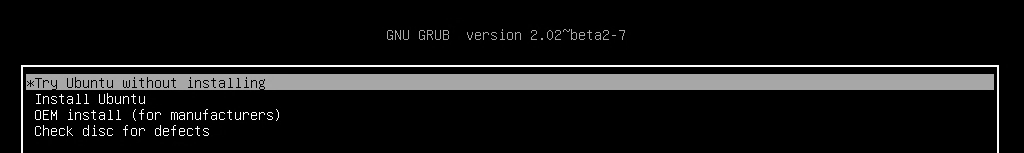
\includegraphics[width=\linewidth]{images/instalacja_UEFI_boot.png}
\end{center}

\noindent Do wyboru masz następujące opcje:
\begin{itemize}
\item \textcolor{ubuntu_orange}{Try Ubuntu without installing (Wypróbuj Ubuntu bez instalowania)} --- Uruchomi system Ubuntu bez instalacji go na dysku twardym. W ten sposób możesz przetestować Ubuntu i zobaczyć jak działa w praktyce. Wszystkie zmiany, jakie wprowadzisz w systemie, zostaną odrzucone po wyłączeniu komputera. Należy pamiętać, że w tym trybie Ubuntu działa bardzo wolno, gdyż musi korzystać z powolnego nośnika (płyta DVD lub pendrive). Po normalniej instalacji Ubuntu będzie działać z pełną wydajnością. Skrót do instalatora systemu znajduje się na pulpicie.
\item \textcolor{ubuntu_orange}{Install Ubuntu (Zainstaluj Ubuntu)} --- Ta opcja bezpośrednio uruchomi instalator Ubuntu bez wczytywania całego systemu.
\item \textcolor{ubuntu_orange}{OEM Install (Instalacja dla producentów sprzętu)} --- Ta opcja pozwala zainstalować podstawowy system bez tworzenia użytkownika. Podczas pierwszego uruchomienia zostaniesz poproszony o stworzenie nowego użytkownika.
\item \textcolor{ubuntu_orange}{Check disk for defects (Sprawdź płytę pod kątem błędów odczytu)} --- Ta opcja sprawdzi, czy używany nośnik został prawidłowo utworzony.\\
Przed przystąpieniem do instalacji systemu warto wykonać sprawdzenie nośnika instalacyjnego. Potrwa to góra kilka minut, a pozwoli zaoszczędzić czas w przyszłości. Podczas przeprowadzania testów komputer może wyświetlać tylko czarny ekran. Jeżeli nie znajdzie żadnych błędów, otrzymasz komunikat \textcolor{ubuntu_orange}{Check Finished: No errors found. Press any key to reboot your system (Zakończono sprawdzanie: nie znaleziono błędów. Wciśnij dowolny klawisz, aby zresetować komputer)}. Po ponownym uruchomieniu komputera możesz przystąpić do instalacji. Jeżeli znaleziono jakiekolwiek błędy, to należy ponownie przygotować nośnik instalacyjny. Użycie wadliwego instalatora doprowadzi do uszkodzenia systemu. 
\end{itemize}
\clearpage
\subsubsection{Uruchomienie instalatora BIOS}
\label{instalacja_uruchomienie}
\begin{wrapfigure}{l}{0.5\textwidth}
	\vspace{-10pt}
	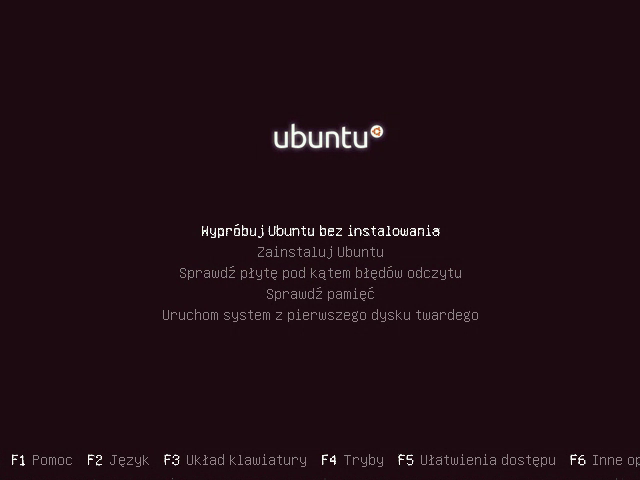
\includegraphics[width=\linewidth]{images/instalacja_BIOS_boot.png}
\end{wrapfigure}

Po wybraniu urządzenia z nośnikiem instalacyjnym komputer rozpocznie proces jego uruchamiania. Może to potrwać od kilku do kilkunastu sekund. W tym czasie ekran komputera będzie czarny, bądź będą się przez niego przewijały napisy. Kiedy ekran komputera zmieni kolor z czarnego na fioletowy, wciśnij dowolny klawisz, aby przejść do ustawień instalatora. Jeżeli tego nie zrobisz, instalator usruchomi się w trybie \textcolor{ubuntu_orange}{Wypróbuj Ubuntu bez instalacji}.

Na początek wybierz język, w jakim system będzie się z tobą komunikował. Przy pomocy klawiszy kursora przejdź do trzeciej kolumny. Język polski znajduje się mniej więcej w połowie tej kolumny. Wciśnij \keys{\returnwin}, aby zatwierdzić.

\begin{itemize}
\item \textcolor{ubuntu_orange}{Wypróbuj Ubuntu bez instalacji} --- Uruchomi system Ubuntu w trybie Live, bez rozpoczynania procesu instalacji na dysku twardym. W ten sposób możesz przetestować Ubuntu i zobaczyć jak działa w praktyce. Wszystkie zmiany, jakie wprowadzisz w systemie, zostaną odrzucone po wyłączeniu komputera. Należy pamiętać, że w tym trybie Ubuntu działa bardzo wolno, gdyż musi korzystać z powolnego nośnika (płyta DVD lub pendrive). Po normalnej instalacji Ubuntu będzie działać z pełną wydajnością. Skrót do instalatora systemu znajduje się na pulpicie.
\item \textcolor{ubuntu_orange}{Zainstaluj Ubuntu} --- Ta opcja bezpośrednio uruchomi instalator Ubuntu bez wczytywania całego systemu.
\item \textcolor{ubuntu_orange}{Sprawdź płytę pod kątem błędów odczytu} --- Ta opcja sprawdzi, czy używany nośnik został prawidłowo utworzony.\\
Przed przystąpieniem do instalacji systemu warto wykonać sprawdzenie nośnika instalacyjnego. Potrwa to góra kilka minut, a pozwoli zaoszczędzić czas w przyszłości. Podczas przeprowadzania testów komputer może wyświetlać tylko czarny ekran. Jeżeli nie znajdzie żadnych błędów, otrzymasz komunikat \textcolor{ubuntu_orange}{Check Finished: No errors found. Press any key to reboot your system} (\textit{Zakończono sprawdzanie: nie znaleziono błędów. Wciśnij dowolny klawisz, aby zresetować komputer}). Po ponownym uruchomieniu komputera możesz przystąpić do instalacji. Jeżeli znaleziono jakiekolwiek błędy, to należy ponownie przygotować nośnik instalacyjny. Użycie wadliwego instalatora doprowadzi do uszkodzenia systemu. 
\item \textcolor{ubuntu_orange}{Sprawdź pamięć} --- Ta opcja uruchomi program Memtest, który wykona test pamięci operacyjnej komputera (RAM). Uszkodzona pamięć jest jedną z częstszych przyczyn błędów instalatora, wpływa również negatywnie na pracę zainstalowanego systemu.
\item \textcolor{ubuntu_orange}{Uruchom system z pierwszego dysku twardego} --- Ta opcja kończy pracę instalatora i uruchamia podstawowy system operacyjny komputera.
\end{itemize}

Dodatkowe opcje widoczne na dolnym pasku uruchamia się wciskając odpowiedni klawisz funkcyjny:
\begin{itemize}
\item \keys{F1} --- Wyświetla pomoc, wraz ze szczegółowym opisem poszczególnych opcji konfiguracyjnych.
\item \keys{F2} --- Zmiana języka instalatora.
\item \keys{F3} --- Zmiana układu klawiatury.
\item \keys{F4} --- Zmiana trybu pracy instalatora:
        \begin{description}
        \item[\textcolor{ubuntu_orange}{Zwykły}] --- Tryb podstawowy, którego właśnie używasz.
        \item[\textcolor{ubuntu_orange}{Użycie nośnika aktualizującego sterowniki}] --- W czasie takiej instalacji zostaniesz poproszony o włożenie dysku CD z aktualnymi sterownikami. Tej opcji używa się, jeżeli aktualnie używany instalator nie obsługuje aktualnego sprzetu. W praktyce lepiej jest nagrać nowszą wersję instalatora.
        \item[\textcolor{ubuntu_orange}{Instalacja OEM (dla producentów sprzętu)}] --- Pozwala zainstalować podstawowy system bez tworzenia użytkownika. Podczas pierwszego uruchomienia zostaniesz poproszony o stworzenie nowego użytkownika.
        \end{description}
\item \keys{F5} --- Pozwala włączyć/wyłączyć dodatkowe opcje, ułatwiające instalację osobom niepełnosprawnym (klawiatura ekranowa, lupa, wysoki kontrast, czytnik ekranu, klawiatura Braille'a).
\item \keys{F6} --- Dodatkowe parametry rozruchu, pomocne w przypadku napotkania problemów ze sprzętem.
\end{itemize}
